\newpage
\subsubsection{W-Wing}
Die Technik \textit{W-Wing} ist die letzte und schwierigste Technik der Wings. Hierbei werden immer zwei Ziffern betrachtet. Zuerst sucht man eine Zelle, in der nur noch zwei Kandidaten x und y möglich sind. Nun wird eine Figur gesucht, in der der Kandidat x nur noch zwei mal vorkommen kann und eines der möglichen Vorkommen von der ersten Zelle ausgeschlossen würde. Im letzten Schritt sucht man eine Zelle, die wieder ausschließlich die Kandidaten x und y enthält und die das andere mögliche Vorkommen der Ziffer x in der zuvor gefundenen Figur ausschließen würde. Findet man eine solche Konstelation, dann handelt es sich um einen \textit{W-Wing}. Gelöscht werden können die  Kandidaten y, die von beiden Zellen gleichzeitig ausgeschlossen werden, da der Kandidat y entweder in der ersten oder in der zweiten gefundenen Zelle stehen muss.

\begin{figure}[h]
\begin{center}
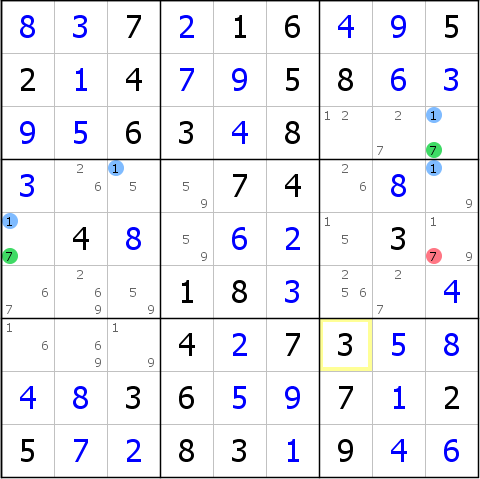
\includegraphics{./img/W_Wing.png}
\caption{W-Wing}
\end{center}
\end{figure}

In \textbf{Abbildung 3.15} betrachten wir zuerst z8s9. Hier finden wir die Ziffer 9 für x und 5 für y. Die gesuchte Figur ist Spalte 8, da hier der Kandidat 9 nur noch zwei mal vorkommen kann und eines der Vorkommen von z8s9 ausgeschlossen wird.
Das andere Vorkommen wird von z4s4 ausgeschlossen. In dieser Zelle befinden sich ausserdem nur noch die Kandidaten x und y. Damit ist die Bedingung für den \textit{W-Wing} erfüllt und der rot markierte Kandidat kann gelöscht werden. Wir betrachten zwei Fälle, entweder die Ziffer 5 steht in z8s9 oder nicht. Im ersten Fall würde der rot markierte Kandidat direkt ausgeschlossen werden. Wenn die Ziffer 5 nicht in z8s9 steht, dann steht dort die Ziffer 9. Damit kann die in Spalte 8 nur noch an Position 4 stehen und damit muss in z4s4 die Ziffer 5 stehen, was wiederum den rot markierten Kandidaten ausschließt. In keinem der Fälle kann der Kandidat dort stehen und wird daher gelöscht..t